\documentclass[12pt]{article}

\usepackage[english]{babel}
\usepackage[utf8x]{inputenc}
\usepackage[T1]{fontenc}
\usepackage{parskip}
\usepackage{lipsum}
\usepackage[a4paper, total={6in, 8in}]{geometry}
\usepackage{setspace}
\usepackage[superscript]{cite}
\usepackage{xcolor}
\usepackage{hyperref}
\usepackage{enumitem}
\usepackage{listings}
\usepackage{amsmath}
\usepackage{amssymb}
\usepackage{ifsym}
\usepackage{tikz}


\begin{document}
	\begin{flushright}
		\today
	\end{flushright}
	{\Large \textbf{Assignment 12}}
	
	{\large Query Optimization}
	
	\textsc{Ilaria Battiston - 03723403} \\
	\textsc{Mareva Zenelaj - 03736071}
	
	\rule{\linewidth}{0.5pt}
	
	\section{First exercise}
	Probability of $0 \leq j \leq 90$ pages being skipped:
	\begin{figure}[h]
		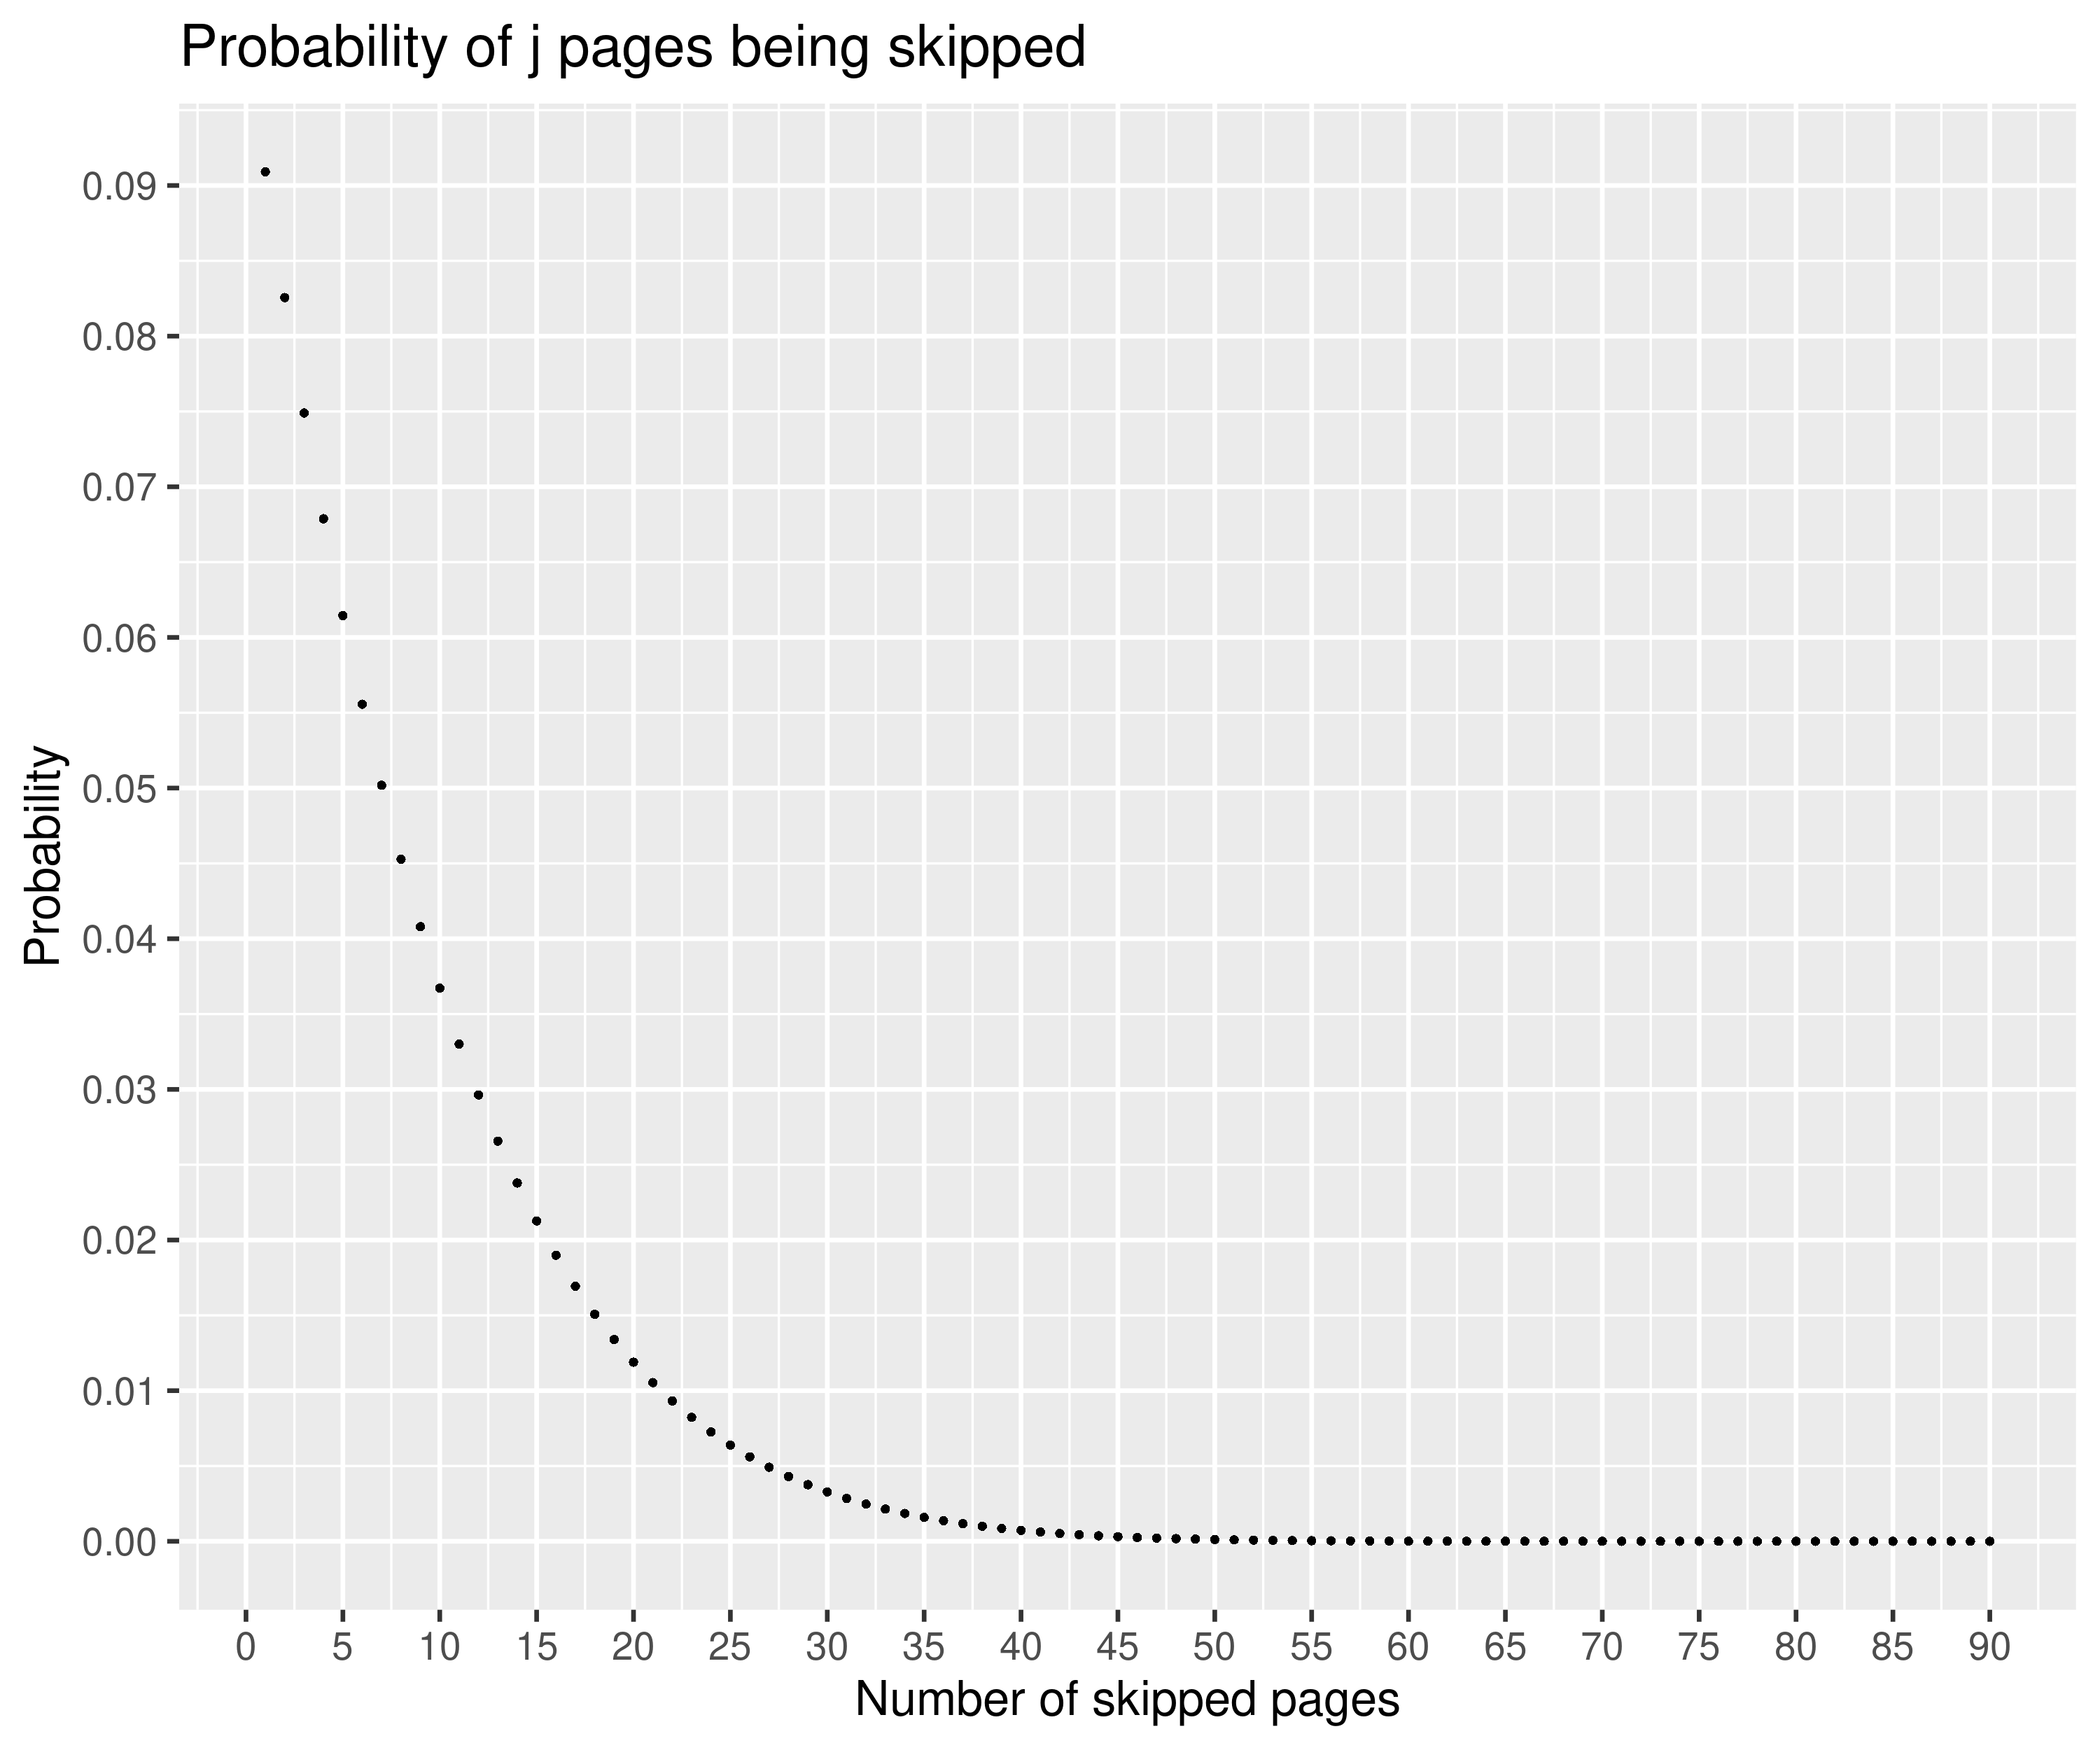
\includegraphics[scale=0.7]{plot_skipped.png}
		\centering
	\end{figure}
	    
	Expected distance between two pages B = 100, b = 10, (10 bits set to 1): computing the distribution of zeros, and the expected number of zeros between two 1s.
	$$\Bar{B}_b^B = \frac{B-b}{b+1} = \frac{100-10}{10_1} = \frac{90}{11} = 8.18$$
	    
	Expected distance between the beginning and the last page to be read:
	$$\Bar{B}_{tot} = \frac{Bb +b}{b+1} = \frac{100*10 + 10}{11} = \frac{1010}{11} = 91.8$$
	    
	Expected distance between the first and the last page
	$$\Bar{B}_{1-span} = \frac{Bb-B+2b}{b+1} = \frac{100 \cdot 10-100+20}{11} = \frac{920}{11} =81.9$$
	
	\section{Second Exercise}
	
	The number of elements for which $R.a \geq 55$ holds true:
	
	$R.a \geq 55$ = $R.a > 55$ + $R.a = 55$
	
	$\frac{60-40}{4} = 5$
	
	5 elements $\implies [55, 60) = 1/4$ of total
	
	0 in the first bucket, 0 in the second, 1 in the third, 2 in the fourth and 0 in the last one. Therefore there are 3 elements.
	
	\section{Third exercise}
	$R.a = S.b$ \\
	When estimating joins on histograms with non-aligned bucket boundaries, buckets are split, such that boundaries are aligned.
	
	Since it is impossible to evenly split buckets with odd numbers, when in doubt the element is placed in the bucket on the left.
	
	\begin{tabular}{c|c|c|c|c|c|c|c}
	     $R.a$ & [0, 10) & [10, 20) & [20, 40) & [40, 50) & [50, 60) & (60, 80] & [80, 100) \\
	     \hline
	     count & 1 & 0 & 3 & 2 & 2 & 2 & 0 \\
	\end{tabular}
	
	\begin{tabular}{c|c|c|c|c|c|c|c}
		$S.b$ & [0, 10) & [10, 20) & [20, 40) & [40, 50) & [50, 60) & (60, 80] & [80, 100) \\
		\hline
		count & 2 & 4 & 1 & 6 & 1 & 2 & 1 \\
	\end{tabular}
	
	$$(R.a = R.b) = \frac{1 \cdot 6 + 1 \cdot 3 + 2 \cdot 6 + 4 \cdot 4}{(1+3+2+4) \cdot (6+1+6+4)} = \frac{37}{170} = 0.217\%$$
	
	$$(R.a = R.b) = \frac{1 \cdot 2 + 4 \cdot 0 + 3 \cdot 1 + 2 \cdot 4 + 2 \cdot 1 + 2 \cdot 1 + 1 \cdot 0}{(1+0+3+2+2+2+0) \cdot (2+4+1+6+1+2+1)} = \frac{17}{170} = 0.1$$
	
	Selectivity of $(R \Join S) \approx 0.1$
\end{document}
